 % The main file for CAMP reports
 % Don't put any content in here.
 % Don't even include content files by using \input or \inlcude.
 % Put your content to TEXT.TEX or include it there using \input.
 % Uses:
 %		SETTINGS.TEX	contains the settings for this document
 %		COMMANDS.TEX	contains commands which can be used while writing
 %		INFO.TEX			contains the author, title and so on for the cover
 %		COVER.TEX			formats the front cover of the document
 %		ABSTRACT.TEX	contains the abstract to be included (if needed)
 %		TEXT.TEX			contains the actual content of the document
 %		BIB.BIB				containt the BibTeX entries for the document
 
 
%% Draft document mode
%% Final document
\documentclass[11pt,a4paper,bibtotoc,idxtotoc,headsepline,footsepline,footexclude,BCOR12mm,DIV13,parskip=full]{scrbook}

%\documentclass[11pt,a4paper,bibtotoc,idxtotoc,headsepline,footsepline,footexclude,BCOR20mm,DIV10]{scrbook}

% KOMA-Optionen:
%  bibtotoc: include bibliography in table of contents
%  idxtotoc: include index in table of contents
%  headsepline: use horizontalline under heading
%  BCOR: binding correcion (Bindungskorrektur) (e.g.: BCOR5mm)
%  DIV: Number of sheet sections (used for layout) (e.g.: DIV12)



% include title and author information for the cover
% Set here the title, authors and other stuff to be used for the cover
% This file is used by MAIN.TEX

% set title, authors and stuff for the cover
\def\doctype{Bachelorarbeit in Informatik}
\def\title{Myriad -- a mailmerge tool for massive parallel, yet individual email conversations}
\def\titleGer{Myriad -- ein Serienbrief Email-Tool f{\"u}r hochgradig parallele, jedoch individualisierte Emailkonversationen}
\def\author{Ludwig Schubert}
\def\date{5. Juni 2013}

% text to appear in the footer
\def\footertext{}


% include settings
% Included by MAIN.TEX

\renewcommand{\sectfont}{\normalfont \bfseries}        % Schriftart der Kopfzeile

% manipulate footer
\usepackage{scrpage2}
\pagestyle{scrheadings}
\ifoot[\footertext]{\footertext} % \footertext set in INFO.TEX
%\setkomafont{pagehead}{\normalfont\rmfamily}
\setkomafont{pagenumber}{\normalfont\rmfamily}

%% allow sophisticated control structures
\usepackage{ifthen}

% use Palatino as default font
\usepackage{palatino}

% enable special PostScript fonts
\usepackage{pifont}

% make thumbnails
\usepackage{thumbpdf}

%to use the subfigures
\usepackage{subfigure}


\usepackage{colortbl}


%% show program code\ldots
%\usepackage{verbatim}
%\usepackage{program}

%% enable TUM symbols on title page
\usepackage{styles/tumlogo}


\usepackage{multirow}

%% use colors
\usepackage{color}

%% make fancy math
\usepackage{amsmath}
\usepackage{amsfonts}
\usepackage{amssymb}
\usepackage{textcomp}
\usepackage{yhmath} % f�r die adots 
%% mark text as preliminary
%\usepackage[draft,german,scrtime]{prelim2e}

%% create an index
\usepackage{makeidx}

% for the program environment
\usepackage{float}

%% load german babel package for german abstract
%\usepackage[german,american]{babel}
\usepackage[german,english]{babel}
\selectlanguage{english}

% use german characters as well
\usepackage[latin1]{inputenc}       % allow Latin1 characters

% use initals dropped caps - doesn't work with PDF
%\usepackage{dropping}
% Don't use the package as it doesn't seem to work by default.

\usepackage{styles/shortoverview}
%----------------------------------------------------
%      Graphics and Hyperlinks
%----------------------------------------------------

%% check for pdfTeX
\ifx\pdftexversion\undefined
 %% use PostScript graphics
 \usepackage[dvips]{graphicx}
 \DeclareGraphicsExtensions{.eps,.epsi}
 \graphicspath{{figures/}{figures/review}} 
 %% allow rotations
 \usepackage{rotating}
 %% mark pages as draft copies
 %\usepackage[english,all,light]{draftcopy}
 %% use hypertex version of hyperref
 \usepackage[hypertex,hyperindex=false,colorlinks=false]{hyperref}
\else %% reduce output size \pdfcompresslevel=9
 %% declare pdfinfo
 %\pdfinfo { 
 %  /Title (my title) 
 %  /Creator (pdfLaTeX) 
 %  /Author (my name) 
 %  /Subject (my subject	) 
 %  /Keywords (my keywords)
 %}
 %% use pdf or jpg graphics
 \usepackage[pdftex]{graphicx}
 \DeclareGraphicsExtensions{.jpg,.JPG,.png,.pdf,.eps}
 \graphicspath{{figures/}} 
 
 %% Load float package, for enabling floating extensions
 \usepackage{float}
 
 %% allow rotations
 \usepackage{rotating}
 %% use pdftex version of hyperref
 \usepackage[pdftex,colorlinks=false,linkcolor=red,citecolor=red,%
 anchorcolor=red,urlcolor=red,bookmarks=true,%
 bookmarksopen=true,bookmarksopenlevel=0,plainpages=false%
 bookmarksnumbered=true,hyperindex=false,pdfstartview=%
 ]{hyperref}
%
%\usepackage[pdftex,colorlinks=false,linkcolor=red,citecolor=red,%
% anchorcolor=red,urlcolor=red,bookmarks=true,%
% bookmarksopen=true,bookmarksopenlevel=0,plainpages=false%
% bookmarksnumbered=true,hyperindex=false,pdfstartview=%
% ]{hyperref}
\fi


\setcounter{tocdepth}{4} 

%% Fancy chapters
%\usepackage[Lenny]{fncychap}
%\usepackage[Glenn]{fncychap}
%\usepackage[Bjarne]{fncychap}

%\usepackage[avantgarde]{quotchap}

% set the bibliography style
%\bibliographystyle{styles/bauermaNum}
%\bibliographystyle{alpha}
\bibliographystyle{plain}


% include commands
% Commands to be used within the TUM report document
% Included by MAIN.TEX
% Please include your own cool commands here. 
% Be only sure to comment it sufficiently so others can use it.

%-------------------------------------------------------------
%                      Own Commands
%-------------------------------------------------------------


%-------------------------------------------------------------
% math stuff -------------------------------------------------

% nice R, N, C
\newcommand{\nat}{\mathbb{N}}
\newcommand{\real}{\mathbb{R}}
\newcommand{\compl}{\mathbb{C}}



% norm
\newcommand{\norm}[1]{\left\| #1 \right\|}

% un demi
\newcommand{\half}{\frac{1}{2}}

% parantheses
\newcommand{\parenth}[1]{ \left( #1 \right) }
\newcommand{\bracket}[1]{ \left[ #1 \right] }
\newcommand{\accolade}[1]{ \left\{ #1 \right\} }
%\newcommand{\angle}[1]{ \left\langle  #1 \right\rangle }

% partial derivative: %#1 function, #2 which variable
% simple / single line version
\newcommand{\pardevS}[2]{ \delta_{#1} f(#2) }
% fraction version
\newcommand{\pardevF}[2]{ \frac{\partial #1}{\partial #2} }

% render vectors: 3 and 4 dimensional
\newcommand{\veciii}[3]{\left[ \begin{array}[h]{c} #1 \\ #2 \\ #3	\end{array} \right]}
\newcommand{\veciv}[4]{\left[ \begin{array}[h]{c} #1 \\ #2 \\ #3 \\ #4	\end{array} \right]}

% render matrices: 3  dimensional (arguments in row first order)
\newcommand{\matiii}[9]{\left[ \begin{array}[h]{ccc} #1 & #2 & #3 \\ #4 & #5 & #6 \\ #7 & #8 & #9	\end{array} \right]}
%DOESN'T WORK,DON'T KNOW WHY \newcommand{\mativ}[16]{\left[ \begin{array}[h]{cccc} #1 & #2 & #3 & #4 \\ #5 & #6 & #7 & #8 \\ #9 & #10 & #11 & #12 \\ #13 & #14 & #15 & #16 \end{array} \right]}


%-------------------------------------------------------------
%-------------------------------------------------------------


%-------------------------------------------------------------
% some abreviations ------------------------------------------
\newcommand{\Reg}{$^{\textregistered}$}
\newcommand{\reg}{$^{\textregistered}$ }
\newcommand{\Tm}{\texttrademark}
\newcommand{\tm}{\texttrademark~}
\newcommand {\bsl} {$\backslash$}

%-------------------------------------------------------------
%-------------------------------------------------------------


%-------------------------------------------------------------
% formating --------------------------------------------------

% Theorem & Co environments and counters
\newtheorem{theorem}{Theorem}[chapter]
\newtheorem{lemma}[theorem]{Lemma}
\newtheorem{corollary}[theorem]{Corollary}
\newtheorem{remark}[theorem]{Remark}
\newtheorem{definition}[theorem]{Definition}
\newtheorem{equat}[theorem]{Equation}
\newtheorem{example}[theorem]{Example}
\newtheorem{algorithm}[theorem]{Algorithm}

% inserting figures
\newcommand{\insertfigure}[4]{ % Filename, Caption, Label, Width percent of textwidth
	\begin{figure}[htbp]
		\begin{center}
			\includegraphics[width=#4\textwidth]{#1}
		\end{center}
		\vspace{-0.4cm}
		\caption{#2}
		\label{#3}
	\end{figure}
}




% referecing figures

\newcommand{\refFigure}[1]{ %label
	figure \ref{#1}
}
\newcommand{\refChapter}[1]{ %label
	chapter \ref{#1}
}

\newcommand{\refSection}[1]{ %label
	section \ref{#1}
}

\newcommand{\refParagraph}[1]{ %label
	paragraph \ref{#1}
}

\newcommand{\refEquation}[1]{ %label
	equation \ref{#1}
}

\newcommand{\refTable}[1]{ %label
	table \ref{#1}
}




\newcommand{\rigidTransform}[2]
{
	${}^{#2}\!\mathbf{H}_{#1}$
}

%code, in typewriter
\newcommand{\code}[1]
 {\texttt{#1}}

% comment that appears on the border - very practical !!!
\newcommand{\comment}[1]{\marginpar{\raggedright \noindent \footnotesize {\sl #1} }}

% page clearing
\newcommand{\clearemptydoublepage}{%
  \ifthenelse{\boolean{@twoside}}{\newpage{\pagestyle{empty}\cleardoublepage}}%
  {\clearpage}}


%-------------------------------------------------------------
%-------------------------------------------------------------


\newcommand{\etAl}{\emph{et al.}\mbox{ }}

\linespread{1.2}

\makeglossary

\begin{document}
	   
	\frontmatter
	
	    % The front cover for the TUM report document.
% Included by MAIN.TEX


%--------------------------------------------------
% The Front Cover
%--------------------------------------------------

% The front cover for the TUM document.
% Included by MAIN.TEX


%--------------------------------------------------
% The Front Cover
%--------------------------------------------------

% correct BCOR - undo at the end !!!
\def\bcorcor{0.15cm}
\addtolength{\hoffset}{\bcorcor}

\thispagestyle{empty}

 \vspace{4cm}
\begin{center}
	       \oTUM{4cm}
	   
	   \vspace{5mm}     
	   \huge FAKULT{\"A}T F{\"U}R INFORMATIK\\ 
	   \vspace{0.5cm}
	 \large DER TECHNISCHEN UNIVERSIT{\"A}T M{\"U}NCHEN\\
    \vspace{1mm}
        
	\end{center}
		

\vspace{15mm}
\begin{center}

   {\Large \doctype}

  \vspace{20mm}
  
  {\huge\bf \title}\\%[3ex]
  
  
  \vspace{15mm}
  
  
  {\LARGE  \author}
  
  \vspace{10mm}
  
  \begin{figure}[h!]
  \centering
   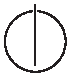
\includegraphics[width=2cm]{styles/in_tum_logo.pdf}
  \end{figure}
  
  \end{center}


	    \clearemptydoublepage
	
	    % The titlepage for the CAMP report document.
% Included by MAIN.TEX


%--------------------------------------------------
% The title page
%--------------------------------------------------

% correct BCOR - undo at the end !!!
\def\bcorcor{0.15cm}
\addtolength{\hoffset}{\bcorcor}

\thispagestyle{empty}

 \vspace{10mm}
\begin{center}
	       \oTUM{4cm}
	   
	   \vspace{5mm}
	   \huge FAKULTÄT FÜR INFORMATIK\\
	   \vspace{0.5cm}
	 \large DER TECHNISCHEN UNIVERSITÄT MÜNCHEN\\
        
	\end{center}
		

\vspace{10mm}
\begin{center}

   {\Large \doctype}

  \vspace{10mm}
  
  {\LARGE \title}\\
  
  
  \vspace{10mm}
  
  
  {\LARGE  \titleGer}\\
  
  
  \vspace{10mm}

    %\hfill
    \begin{tabular}{ll}
	   \Large Author:     & \Large \author \\[2mm]
	   \Large Supervisor:    & \Large Prof. Dr. Johann Schlichter \\[2mm]
	   \Large Advisor:	& \Large Dr. Wolfgang Wörndl \\[2mm]
	   \Large Date:       & \Large September 30, 2013
	 \end{tabular}
	 
	 \vspace{5mm}
	 
	 \begin{figure}[h!]
  \centering
   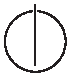
\includegraphics[width=2cm]{styles/in_tum_logo.pdf}
  \end{figure}
   

\end{center}

% undo BCOR correction
\addtolength{\hoffset}{\bcorcor}

	
	    \clearemptydoublepage
\addcontentsline{toc}{chapter}{Disclaimer}

\thispagestyle{empty}
\selectlanguage{german}
	
	\null
	\vfill
	
	\noindent
	Ich versichere, dass ich diese Bachelorarbeit selbständig verfasst und nur
	die angegebenen Quellen und Hilfsmittel verwendet habe.
	
	\vspace{15mm}
	\noindent
	München, den 30. September 2013 \hspace{5cm} \author
\selectlanguage{english}
\newpage

	
	    % Abstract for the TUM report document
% Included by MAIN.TEX


\clearemptydoublepage
\phantomsection
\addcontentsline{toc}{chapter}{Abstract}

\vspace*{1cm}
\begin{center}
{\Large \bf Abstract}
\end{center}

This thesis introduces the myriad system for email mass communication.

Despite its age, Email has remained the prevalent form of electronic communication, it's usage being wildly different from how it was imagined. The tools to handle it, however, are still stuck in their original UI metaphors.

Myriad aims at producing personalized communication on a comparable level to manually composed messages, while reducing user effort.
A cross-over of mailmerge and customer support/helpdesk software, it enables managing big volumes of bidirectional email-based communication.
It is based on a self-developed framework for separating information extraction, decision making, and personalization steps in communication.

The myriad system consists of a server component that handles interfacing with email servers, a core logic system and a web frontend for users.

It can be tested at \url{http://myriad.ludwigschubert.de}.

\vspace*{1cm}
\begin{center}
{\Large \bf Keywords}
\end{center}

Email, Workflow, Helpdesk, Mailmerge, Crowdsourcing, Personalized Communication, Assisted Templating, Generated Documents, Web-Application

\vspace*{1cm}

\begin{figure}[h!]
\centering

\includegraphics[height=2.5cm]{figures/myriad-logo.pdf}
\end{figure}

    	\clearemptydoublepage
\phantomsection
\addcontentsline{toc}{chapter}{Acknowledgements}	


%\chapter*{Acknowledgements}

\vspace*{2cm}

\begin{center}
{\Large \bf Acknowledgments}
\end{center}

\vspace{1cm}




If someone contributed to the thesis... might be good to thank them here.

        \clearemptydoublepage
\phantomsection
\addcontentsline{toc}{chapter}{Table of Contents}

\tableofcontents

  
	\mainmatter
	
	
		% ---------------------------------------------------------------------------
		%
		% Main Matter
        %
		% ---------------------------------------------------------------------------
        \part*{Main Matter}
        \addcontentsline{toc}{part}{Main Matter}
        \chapter{Introduction}
\label{chapter:Introduction}

This chapter gives an overview of the work, arguments for the relevance of new Email tools, as well as the goals pursued by this thesis. Concluding, the structure of the work is explained.

\section{Motivation}

The total number of worldwide email accounts -- 3.3 billion as of 2012 \citep{emailreport} -- indicates how email still is the primary means of asynchronous online communication, despite continued efforts from corporations for successor technologies. \\
While specialized tools, e.g. Facebook's Events or Doodle, can provide a better experience, email is still the ubiquitous fall-back medium that everybody can access. It's non-centralized approach, relying only on deeply embedded infrastructure like the DNS system, has allowed email to become bigger than any proprietary tool.

Thus it is unsurprising that email is used a lot as an organizational tool instead of the mere letter-like two person communication medium that it was set out to be. In fact, use of email as an organizational tool is primed to become even more prominent, with most of the growth and traffic in email usage coming from the corporate world. \citep[p. 3]{emailreport} A person might use email to figure out a good time for a meeting, soliciting comments on his work, or even just organizing a party.

In all of the scenarios mentioned above, the user has to make a trade-off between effort and personalization -- writing individual emails versus sending out a mass mail.

Now, there are lots of benefits of personalized emails. A higher response rate is one of the basic ones. Some scenarios require personalized information as part of the email in order to be effective, e.g. a grade report. Sometimes a personally addressed email is just a lot more likely to produce the desired result \citep[p. 1375, 1380]{emailsalutation}, as it increases perceived social pressure.

In observing one instance of such a usage of email, a recruitment campaign for a scientific study, we observed a lot of duplicated efforts, inconsistent communication and overall potential for tool assistance.\footnote{See \autoref{section:FunctionalAnalysis}.} We set out to develop a mail merge system that didn't require complicated desktop software, yet was more powerful and workflow oriented than previously available mail merge software.\footnote{See \autoref{section:MailmergeSystems} for a more in-depth comparison with pre-existing systems.}

\section{Goals}

We developed a web-based email client with mail merging capabilities for massive parallel, yet personalized email conversations, Myriad. The focus of Myriad lies not on traditional, individual email based replies. Instead, it aims to provide tools that allow managing big amounts of similar emails efficiently.
To fulfill this goal, Myriad provides a high level organizational abstraction called \code{Campaigns}, a visualization of individual conversations' state and actionability, filtering and actions on groups of results, easy reusability and automation of replies (\code{Messages}), as well as support for delegation to assistants and generally usable integration into existing email and information management infrastructure.
Those simple, combinable features are supposed to enable users' email workflows to be both personalized and well-organized, while reducing manual and duplicated effort. To define a simple goal for ourselves we created \autoref{figure:EffortVSPersonalization}, which plots user effort against personalization for an email campaign. The lower, left-hand corner is exemplified by a single mass mail: barely any personalization at minimal effort. The upper, right-hand corner shows writing every email by hand: maximum personalization, but at a high effort. Myriad's goal is to end up below the drawn line; achieving the desired degree of personalization at sublinear effort.

\insertfigure{figures/effort_vs_personalization.pdf}{Myriad's goal is to achieve a desired degree of personalization at sublinear effort.}{figure:EffortVSPersonalization}{0.25}

\section{Collaboration}

This thesis is based on research I conducted together with \href{mailto:ikas@in.tum.de}{Christian Ikas}, \href{mailto:boztop@gmail.com}{Barış Öztop} and \href{mailto:nicolas@cs.stanford.edu}{Nicolas Kokkalis}. To avoid overlap between the researchers, I will focus on the system design process, architecture and implementation details. Those were my main responsibilities in the project.

For a more in-depth look at the motivation for the project, the comparison with existing systems and the relevance for survey research, see Barış Oztop's master thesis.\\
For a more business-process focussed look at email workflow tools, see Christian Ikas' master thesis.

\section{Outline}

\textbf{This chapter} gives an overview of the work, and arguments for the relevance of new Email tools, as well as the goals pursued by this thesis. Concluding, the structure of the work is explained.

In \textbf{\autoref{chapter:Technical}}, \textbf{\nameref{chapter:Technical}}, relevant technical background information is provided. The decision to build a web app is motivated. Standard-compliant email systems are explained and relevant standards are introduced. Lastly, an introduction to workflow systems and historic examples is given.

In \textbf{\autoref{chapter:Comparison}}, \textbf{\nameref{chapter:Comparison}},  two major categories of software -- dedicated mail merge systems, and customer support systems -- are introduced, which overlap in functionality with Myriad.

In \textbf{\autoref{chapter:Concept}}, \textbf{\nameref{chapter:Concept}}, the architecture of the proposed system is motivated and its design process is highlighted.

In \textbf{\autoref{chapter:Implementation}}, \textbf{\nameref{chapter:Implementation}}, is concerned with technical details of how Myriad was implemented. The collaborative development process is described, as are actual system component and their functionality.

In \textbf{\autoref{chapter:Evaluation}}, \textbf{\nameref{chapter:Evaluation}}, Myriad's initial goals will be reiterated and contrasted with real world observed usage.

In \textbf{\autoref{chapter:Conclusion}}, \textbf{\nameref{chapter:Conclusion}},  the relevance of this system and the proposed framework is discussed; future work is outlined and possible directions proposed.

This is followed by a \textbf{\hyperref[chapter:Bibliography]{Bibliography}} of cited works and a \textbf{\hyperref[chapter:Figures]{List of Figures}}.

The \textbf{\nameref{part:Appendix}} contains selected source code examples, the development of the system design over time in UML Diagrams, and a \textbf{\nameref{chapter:Colophon}}.


		\chapter{Technical Background}
\label{chapter:Technical}

This chapter provides relevant technical background information. It motivates the decision to build a web app. Standard-compliant email systems are explained and relevant standards are introduced. Lastly, it gives an introduction to workflow systems and provides historic examples.

\section{Web Applications}

This section comprises an introduction to web applications and their development. It lays the foundation for the implementation details of the Myriad system in chapter \autoref{chapter:Implementation}.

Web applications, or, more precisely, \emph{web-based applications}, don't have a strict formal definition, but here the term is used in its common meaning\cite{webapptrends}: an application, which is accessed through a web browser. Unlike a traditional computer program that is usually written in a single programming language, compiled and then executed on a computer, a web application consists of many interoperating systems and programs, commonly not even run on the same machine. \footnote{While the distributed, non-homogeneous nature of web applications makes their development process more complex, it also afforded me the opportunity to learn about the full spectrum of the current unix eco-system.}

Traditionally, a website is comprised of static \gls{html} files and \gls{css} markup to display its content. To support the dynamic nature of user-specific \em{applications} rather than \em{documents}, a typical approach is to generate the \gls{html} files dynamically at request time. Together with client side executed javascript, this supports more interactivity. This is the current standard for many web development frameworks such as Ruby on Rails, Django or PHP.

Future Web Applications will most likely go further in their separation of concerns, shifting the application logic to the client side. With frameworks such as Sproutcore, which are served statically and execute all business logic on the client side in javascript while relying on the server mainly as a data source, one can already see the beginnings of this clearer, more mature development paradigm. As of the time of writing however\footnote{ \today }, the model of dynamically rendered \gls{html} files is still prominent. With larger communities and good documentation it is the de-facto standard of web application development.

\subsection{Software Stacks}

The client-side stack includes the webbrowser and javascript engine to interpret the \gls{html} and Javascript files from the webserver.

The server-side stack is tradtionally an assortment of tools, starting with an HTTP server such as |Apache| or |NginX|, which handle static file serving. The HTTP server forwards requests for dynamic content to a web server, such as |fast_cgi| or |Unicorn|. These may optionally have a middleware handler for web middlewares such as |Rack|, or forward directly to the web framework, which handles the business logic, database connections, etc.

Apart from this primary web stack many web applications rely on additional services running on the backend server. A simple example would be an additional Key-Value store for caching purposes, such as |Redis| or |MongoDB|. But infrastructure software, such as the common unix scheduler |cron|, backup tasks, SMTP servers, or background workers, are also part of the backend stack. All of these parts contribute to the end result and have to be managed and integrated in a process called deployment. The solution I chose for automating deployment is explained in \autoref{subsection:Deployment}.

\subsection{Ruby on Rails}



\insertfigure{figures/rails_architecture.png}{Ruby on Rails Architecture Diagram}{RailsArchitecture}{.75}{Picasa User ``Niwatori''}


\section{Email}


\subsection{RFC 2822}

Email is standardized as the ``Internet Message Format'' in RFC 2822\cite{email}.

\subsection{IMAP \& SMTP}

Hello \gls{imap}.


\section{Workflow Systems}


\subsection{History of Workflow Systems}


\subsection{Famous Examples}
		\chapter{Comparison with similar systems}
\label{chapter:Comparison}

In this chapter two major categories of email software which overlap in functionality with Myriad -- mail merge systems, and customer support systems -- are introduced.

Mailmerge systems focus on reaching a big target audience by providing personalization and technical tools for large email campaigns.
Customer support systems are focussed on individuals and their conversations with the user.

To gain these insights we examined a selection of services and products based both on recommendations from peers and freely available online reviews. These were sorted according to received web traffic\footnote{\url{https://www.compete.com}, \url{http://www.alexa.com}, \url{http://www.google.com/trends}}. Rather than the individual services, the categories of those services will be contrasted.

\section{Mail Merge Systems}
\label{section:MailmergeSystems}

Mail merge systems automate the process of taking data, such as from a table or a database, and using it to personalize a prewritten template for multiple recipients. An example of this is sending out an email that allows a user to reset their password, but also an automatically generated marketing email, which includes the recipient's name in the greeting.

Mail merge systems often contain advanced templating languages as described by \citet{mailmergeprogramming}. These contain placeholders, such as |first\_name| or |greeting|, but sometimes also offer conditional text -- usually through |if| statements -- and other control flow tools that are familiar from imperative programming languages. These tools focus on sending a large number of emails with enough personalization to get them through spam filters.

\subsection{Email Marketing Services}

Email marketing services use a mail merge system, usually in combination with \gls{html} templates and tracking functionality, to send commercial advertising to large groups of recipients. Most such services allow to create mass emails with a high degree of sophistication. Paired with straightforward import and management of contact lists, these capabilities allow users to put together an email campaign easily. However, these campaigns do not strive to appear as individual conversations -- that they are sent out to a large number of people is widely understood by their recipients. Campaigns initiated by those services are not meant to be bidirectional, and no software support exists in typical email marketing services for handling incoming replies.

Popular examples include iContact\footnote{\url{http://www.icontact.com}} and MailChimp\footnote{\url{http://mailchimp.com}}.

\subsection{Email Delivery Services}

End-user email providers employ a variety of tactics to assign incoming emails a \gls{spam} score, and classify unwanted emails as such. The consequence of that is that a freshly connected \gls{smtp} server which suddenly starts sending a large amount of emails will quickly be classified as a \gls{spam}mer and be blocked.

Thus a market opportunity arose for email delivery services. They account for commonly known \gls{spam} filtering techniques and rent their infrastructure to clients who want to send large amounts of email. Those email delivery providers guarantee a certain level of relevance of emails they send out, while circumventing as many \gls{spam} filtering criteria as possible.

One of them is \gls{dns} whitelisting, a service provided by dnswl.org\citep{dnswl}. \gls{dns} whitelisting means that email providers query a list from dnswl.org to check whether the email server sending an email is whitelisted, which means it has shown not to send \gls{spam} in the past, or at least quickly mitigated any such case. Email delivery services have continuously shown to adhere to these practices in the past, and are consequently usually whitelisted.

Other practices offered include the ``warming-up'' of an \gls{ip} address -- or simply using a shared one -- various authentication protocols on top of \gls{smtp} and plainly monitoring outgoing emails for their \gls{spam} score before actually sending them.

Popular examples of email delivery services include Amazon's \acrfull{ses}\footnote{\url{http://aws.amazon.com/ses/}}, and SendGrid\footnote{\url{http://sendgrid.com}}, both of which offer the practices described above.

\section{Customer Support Systems}

Customer support systems can be divided into two categories, even though their functionality overlaps: \gls{crm} software, which focusses on the holistic view of a recipient over time and communication channels, and helpdesk software, which usually focusses on a ticket-level view of a customer, helping to solve a single issue that prompted the customer to initiate communication. This categorization is mostly historical, with modern helpdesk software offering a lot of \gls{crm} functionality as well.

\subsection{CRM Software}

\acrlong{crm} software focusses on establishing a shared history of interaction with a customer, potentially across multiple channels. With, for example, the establishment of social media as viable communication platforms for companies, \gls{crm} software has evolved to include these channels. Thus it is meant to create a holistic view of interactions with the customer, aiming at making marketing more relevant. A simple example would be recording a customer's choice of beverage on first contact, and rereading this information before a second meeting. In a more digital example it could include extracting a users buying preferences from their order history and using this information for a targeted email marketing campaign. Putting a heavy focus on contact management, \gls{crm}s are geared towards holistically managing customer contact rather than focusing on content in individual conversations.

\gls{crm} software has steadily moved to \gls{saas} models in the last years, with 83\% of all companies expecting to switch to it eventually.\citep{saasindustryreport}

Popular examples of \gls{crm} software include Salesforce\footnote{\url{https://www.salesforce.com}}, and SugarCRM\footnote{\url{http://www.sugarcrm.com}} -- which is available as a self-hosted, free ``community edition''. Market leaders for customized CRM solutions are SAP\footnote{\url{http://global.sap.com/germany/solutions/business-suite/crm/index.epx}} and Oracle\footnote{\url{http://www.oracle.com/us/solutions/crm/overview/index.html}} according to \citet{gartnercrm}.

\subsection{Helpdesk Software}

Helpdesk software is used after a customer has initiated a conversation by writing to a public email support address, or similar systems like forums. This creates a so called ``ticket'' in the helpdesk system. This ticket tracks the status of the customer's inquiry, and is  assigned to a person who is now responsible for it. The tool support of helpdesk software often includes a knowledge base for the workers, response templates to common inquiries, and workflows for escalating tickets to more senior workers. While some helpdesk software does allow for merging similar tickets, they generally focus on individual conversations, which limits their ability to minimize work redundancy.

Popular examples of helpdesk software include ZenDesk\footnote{\url{http://www.zendesk.com}} and desk\footnote{\url{http://www.desk.com/help-desk/software}} -- a Salesforce product.


\section{Summary}

\begin{table}\label{similar}
\ra{1.5}
\centering
\begin{tabular*}{\textwidth}{@{}@{\extracolsep{\fill}}ll@{}lll@{}ll@{}}
  \toprule
  \phantom{} & \phantom{} & \multicolumn{2}{@{}l}{ \textbf{Mail Merge Systems}} & \phantom{} & \multicolumn{2}{@{}l}{ \textbf{Customer Support Systems}} \\
  \cmidrule{3-4} \cmidrule{6-7}
  \emph{Feature} & \phantom{a} &  Email Marketing & Email Delivery & \phantom{a} & CRM       & Helpdesk \\
  \midrule
  Templates       & \phantom{} &  Yes          & n/a        & \phantom{} & Sometimes    & Sometimes   \\
  Reusability     & \phantom{} &  Yes          & n/a        & \phantom{} & Sometimes    & Yes   \\
  Placeholders    & \phantom{} &  Yes          & n/a        & \phantom{} & Sometimes    & Sometimes   \\
  Auto-Responders & \phantom{} &  n/a          & n/a        & \phantom{} & Sometimes    & Yes   \\
  Import Contacts & \phantom{} &  Yes          & n/a        & \phantom{} & Yes          & n/a         \\
  Incoming Email  & \phantom{} &  No & n/a        & \phantom{} & Sometimes    & Yes   \\
  Status Tracking & \phantom{} &  Read/Unread  & n/a        & \phantom{} & No           & Yes   \\
  Sharing         & \phantom{} &  n/a          & n/a        & \phantom{} & Yes          & Yes   \\
  Mass Email      & \phantom{} &  Yes          & Yes        & \phantom{} & No           & No   \\
  \bottomrule
\end{tabular*}
\caption{A comparison of similar systems}
\end{table}

The table above gives a comparison amongst the different systems. Our main finding was that individual products were highly evolved in their support of specific use cases. They all specialized on individual aspects of communication. There were no general purpose tools for handling both incoming and outgoing emails, no products with focus on data collection, and no general purpose tools.

		\chapter{Concept}
\label{chapter:Concept}

In this chapter the architecture of the proposed system is motivated and its development process is highlighted.

\section{Functional Analysis}
\label{section:FunctionalAnalysis}

\section{Product Functions}

\section{User Interface}

\subsection{Prototyping Approaches}

\section{Technical Analysis}

\subsection{Runtime Environment}

\subsection{Server Software Stack}

\subsection{Client Side}

\subsection{Backend Service Connections}

\subsubsection{Google Mail}

\subsubsection{Google Docs}


\section{System Design}

\subsection{Database Schema}

\subsubsection{Unusual Patterns}

\subsection{Distribution of System Components}





		\chapter{Implementation}
\label{chapter:Implementation}

This chapter is concerned with technical details of how Myriad was implemented. The collaborative development process is described, as are actual system components and their functionality.

\section{Preparation and Tools}



\subsection{Development Environment}



\subsection{Collaborative Development}



\subsubsection{\code{git}, \code{gitflow} and Github}



\subsection{Deployment}
\label{subsection:Deployment}



\subsubsection{Deployment Tool \code{Capistrano}}




\section{Server Component}


\subsection{Workers and their Jobs}


\subsection{Maintenance and Rake Tasks}


\pagebreak
\section{Architecture}

Myriad is built around the interaction of five model level concepts, implemented as model classes, and a set of assisting subsystems.
|Campaigns|, which have a set of |Email|s and a bunch of |Contact|s as recipients. The relation between the campaign and the contacts is called |Conversation|; the relation between campaign and the emails is called |Template|.

The shown class diagrams follow a subset of the UML 2.0 class diagram standard\cite{uml}. Since these diagrams are primarily focussed on Myriad's data model, they are first and foremost Entity Relationship diagrams. They are simplified for illustrative purposes and do not constitute an exact specification.

\insertfigure{figures/cd_main.pdf}{Myriad is built around the interaction of 5 model level classes.}{CD-Main}{1}


\subsection{Contact}

Contacts are the names and email addresses of the people you want to email.
They are created when importing from spreadsheets, when typing an email address into a To: field, or when importing existing emails by adding a Gmail label to them. Contacts belong to users. This means that there is only one fred@gmail.com for each user and this fred@gmail.com may be linked to multiple campaigns of that user.

\subsection{Template}

Templates are prototypes of emails. They consist of body text that can contain placeholders, a subject, actions that are triggered when they are sent, and rules that can send them automatically.

\subsection{Email}

Emails are instantiations of Templates. Their body doesn’t contain placeholders anymore, but only the merged email body. They have a delivery status, for example, and keep lots of information on their external representations, like a \code{message\_id}, UIDs for IMAP folders, thread IDs (THRIDs) for Gmail, etc.

\subsubsection{FetchedEmail}

|FetchedEmail| represents Emails that were fetched as raw data from an IMAP server. |FetchedEmail|s encapsulate their respective |RawMail|s.

\subsubsection{IncomingFetchedEmail}

|IncomingFetchedEmail| represents an email from someone else than the user that was fetched from an IMAP server. E.g.: responses from recipients.

\subsubsection{OutgoingFetchedEmail}

|OutgoingFetchedEmail| represents an email the user wrote themselves, but that was fetched from an IMAP server. E.g.: Emails the user wrote in their personal email client, but still in response to recipients of a current campaign.

\subsubsection{CreatedEmail}

|CreatedEmail| represents Emails that were created by Myriad. They don't have a Rawmail, but |CreatedEmail| provides functionality for serializing to a raw text representation.

\subsubsection{OutgoingCreatedEmail}

|OutgoingCreatedEmail| represents an email the user wrote as a message template  and was later generated by Myriad.

\subsubsection{IncomingCreatedEmail}

This class is not implemented yet. While, at first sight, it might seem like an \emph{incoming} email could never be \emph{created} by the system, this could be used for a multitude of plausible scenarios, such as sending persistent messages to the user (instead of the more ephemeral on-screen notifications), importing emails from a non \code{IMAP} compatible email server, or even integrating a chat system, making incoming chat messages appear as emails to the system.

\subsection{Campaign}

Campaigns are a collection of templates and meta information like a connected Google Drive spreadsheet. They additionally contain a list of Keys. You can think of keys as column headers in a spreadsheet.

\subsection{Conversation}

Conversations are like email threads in gmail, but scoped to a specific campaign and contact. They contain all the emails a contact wrote or received within a campaign.

\subsection{Key \& Value}

\insertfigure{figures/cd_key_value.pdf}{Key and Value together allow for storing arbitrary information about a contact in a campaign.}{CD-Key-Values}{1}

One goal of a campaign can be the collection of information. For that, users create a data schema made up of Keys, that they (or somebody they share the campaign with) fill with Values. The Keys consist of a name – the header of the spreadsheet column – while values have a content – the content of a spreadsheet cell in the row of the contact they belong to.
\pagebreak
\subsection{Rules \& KeyBinding}

\insertfigure{figures/cd_rules.pdf}{Rules rely on different ``bindings'' to define their matching criteria.}{CD-Rules}{1}

Searches allow users to constrain the set of all conversations to a subset of them by defining criteria those conversations match. Each search consists of zero or more KeyBindings, zero or more TemplateBindings, as well as an optional conversation status constraint. A KeyBinding is a value that a key must have to satisfy a specific search. Similarly, a TemplateBinding tb of search s specifies a Template t such that a conversation c matches s if c contains an email e, and e is an instantiation of t.
For example, a search might specify that a conversation should be unread to be part of the search’s results. But we also want to allow users to specify constraints on their own Keys, e.g. coming? = “yes”. For that, we needed a flexible way to specify those constraints. So we came up with the concept of a KeyBinding; it “binds the free Key variable to a specific value”. So a KeyBinding associates a search with a Key that contains a specific value (todo: add comparison operators. e.g. age > 21).
Note that Searches are saved to the database. If they specify a template to be sent, we consider them to be “Rules” that can be automatically triggered. Otherwise they just clutter up the database and should eventually be purged by a cronjob. This persisting of searches could be used to remember recent searches.

\pagebreak
\subsection{ValueSettingActions}

\insertfigure{figures/cd_actions.pdf}{ValueSettingActions allow a template to set a certain Key's value to a predefined value. Together with Rules, this allows for custom, state-machine-like behavior specification.}{CD-Actions}{1}

\subsection{Notification}

Notifications are used to “notify” but not only. They also hold state (e.g. invalid user credentials) that can be used only internally by the system (e.g. to avoid syncing emails from users with invalid credentials). They are like “state” descriptors of other objects and in some cases these are visible to the users (e.g. we are syncing your spreadsheet), in other cases only the backend uses them. So maybe they should be called differently. (any ideas?)

They’re an abstract class that we might have taken a little too far. They basically contain a polymorphic Type field, and an ID. Then, madness ensues as we use this information to attach Notifications to any ActiveRecord::Base object in our database. There is a whole class hierarchy beneath Notification, containing classes like ErrorNotification, which uses aforementioned feature to attach Errors or warnings to basically anything. There are also very specific subclasses like TemplateSentToSearchResultsActivityNotification, which are used to notify users. Another example would be a SpreadsheetSyncingNotification, which is also used to inform users. You can define groups of Notification Subclasses that are displayed in different parts of the UI, for example on the Admin Dashboard or on top of the screen for the respective user, as a kind of persistent flash message.

\subsubsection{ActivityNotification}

These are used to display the activity stream, which is currently woefully underdeveloped.
They could also be used to record Assistant actions in the future. Maybe they could even be tied to resources to enable tracking of the last spreadsheet sync, etc.

\subsubsection{UnexpectedStateNotification}

We used these to make sure that all of those little instances where you’re writing a case statement without a default, expecting values to be of a certain type, etc *actually* never occur. And in reality, of course, they do. So if you’re almost certain a certain state should not be reached in a program, put an UnexpectedStateNotification there and be grateful when, two months later, your admin dashboard informs you that what you had deemed impossible happened 6,000 times last night.

\subsubsection{ExceptionNotification}

A simple way to “save” an exception for review from the Admin Dashboard. (Todo: Also save the stacktrace with these, so they might be even more useful.)

\subsubsection{ErrorNotification}

These might be named a little badly, since they can actually mean anything that is attached to a certain resource and might be resolved later on. For example, we could use these to implement an InvalidCredentialsErrorNotification. When, at a later point, the credentials work again, we’ll be able to call InvalidCredentialsErrorNotification.resolve and pass it the user object, deleting the InvalidCredentialsErrorNotification.
An example where these are used to notify not about an error, but simply about a state that’s attached to a resource is the SpreadsheetSyncingNotification.
A possibly better future name might be PersistentNotification or ResourceNotification.


\section{Backend Services Connection}



\subsection{Email Fetching}

As we spent a lot of time figuring out the intricacies of the Gmail IMAP implementation and the manifold cases that can occur when normal (or heavy) users go about their daily email business without considering the restrictions of poor Myriad, we want to spare you repeating the same. We hope to have brought the fetching and email creation logic to a relatively stable state, yet we are certain there remain a bunch of holes that could cause failures in edge cases.
If you do not need to touch the code, you might find the following explanation too detailed, so you shouldn't waste your time with it (bar this overview section). For anybody working with the fetching code, however, the following information should prove very useful - especially if you are unfamiliar with email headers, IMAP protocol details and the like.
In brief, our fetching process works as follows:
1.	Identifying emails on the Gmail server: First, we connect to the user's Gmail account and identify the UIDs (one of many types of email identifiers, see below for a more detailed explanation) of all emails we want to fetch. We use multiple different queries for that, which will later be explained in more detail. Before we move on to the next step, we filter out emails in our database whose UIDs we already know, i.e. have fetched before.
2.	Fetching and processing email data: For the remaining UIDs, we fetch the corresponding email from Gmail, create a Mail object (from the mail gem) for it and determine its type – IncomingFetchedEmail, OutgoingFetchedEmail, etc.
3.	Email creation in Myriad: As a last (but not trivial) step we try to use the information from the Mail object to create an Email object in Myriad.

\subsubsection{IMAP IDLEing}



\subsection{Google Docs Syncing}




\section{``Interesting Practices''}

During the development process we discovered a set of ``Interesting Practices''\footnote{A wordplay on ``Best Practices'', an overused term to describe methods or practices that have produced good results repeatedly.} that didn't seem to fit into any specific software development methodology.

\subsection{Lean Workers with AbstractWorker}

When faced with the task to build a DRY function to start worker threads for all workers, there was no simple way. Additionally, each worker needed a queue name as configuration. Having learned from ActiveModel, I built |AbstractWorker|. It takes care of generating queue names from the class names of it’s subclasses. The descendants method, which returns all subclasses, can be iterated over. This allows starting a worker thread for every queue. It also allowed extracting the ResqueDirector plugin into AbstractWorker, which starts those workers automatically in our Development environment. So one can simply subclass AbstractWorker and rest assured that worker threads will be started for the new subclass automatically, both in development and in production.

\subsection{A small, fixed set of core extensions}

A dynamic language like ruby makes it trivially easy to reopen core classes.\footnote{By simply redefining a class one can extend it.} While initially this seems like a convenience, it's easy to lose track of already implemented extensions. One risks colliding method names\footnote{Ruby 2.0 finally fixed this by introducing \emph{refinements}, a way to extend classes namespaced to the current module.} and reusability is higher if the extension is packaged as a module which is then included where needed.

However, we did decide to keep a set of our extensions, which we felt were both useful and idiomatic. Here's a list of them, together with explanations why we kept them even through multiple code cleanups:

\subsubsection{String}

\begin{description}

\item[remove\_all\_whitespace] A common task when interfacing with APIs, especially when interfacing with IMAP where one can't use a proper parser. This came up multiple times during development, and a commonly suggested solution is to use regular expressions, like so: |gsub /\s+/, ''|. While working perfectly fine, we wanted a more expressive name. This was left as an extension because similar whitespace altering functions like |#strip| or  |#squish| are also declared directly on |String|.
\\
\begin{lstlisting}
  "  This is a string  !   ".remove_all_whitespace
   => "Thisisastring!"
\end{lstlisting}

\item[similar\_to?] A custom equivalence class on |String|s, which are similar if one only considers numbers and downcased letters. This is used to match placeholders with spreadsheet column headers, for example.
In our experience users often used ``First Name'' instead of ``first\_name'' and we wanted to offer an equivalence class that was sufficiently big, while avoiding being totally fuzzy.
\\
\begin{lstlisting}
  "first_name".similar_to? "First Name"
   => true
\end{lstlisting}

\item[ellipsisize] Takes a string and information on how how much of it to keep. It adds an ellipsis where the string was cut off. We used it in many places throughout the interface, for example for only displaying the first line of a collapsed email.
\\
\begin{lstlisting}
  "Supercalifragilisticexpialidocious".ellipsisize
  => "Sup...ous"
\end{lstlisting}


\item[to\_bool] Once again an indication of working with badly specified protocols. This was needed after some Javascript libraries apparently disagree about how to encode |true| in a \gls{url} parameter.
\\
\begin{lstlisting}
  ['true', 't', 'yes', 'y', '1'].map(&:to_bool).all?
  => true
  ['false', 'f', 'no', 'n', '0'].map(&:to_bool).none?
  => true
\end{lstlisting}

\end{description}

\subsubsection{Hash}

\begin{description}

\item[deep\_find] This does a deep traversal of a Hash, looking for any key that matches the argument of this method. When working with APIs that return structured data the format is usually fixed, but we experienced slight inconsistencies for Google's different versions of its OAuth APIs. Of course this method will run into trouble if a key occurs multiple times, but when used in the right places, it makes parsing structured responses incredibly solid.
\\
\begin{lstlisting}
  nested_hash
  => {
      "a key"=>"a value",
      "a nested hash" =>
      {
        "another key"=>"another value",
        "the key"=>"the value"
      }
     }

  simple_hash
  => {
      "another key"=>"another value",
      "the key"=>"the value"}
     }

  simple_hash.deep_find "the key"
  => "the value"

  nested_hash.deep_find "the key"
  => "the value"
\end{lstlisting}

\end{description}

\subsubsection{Array}

\begin{description}

\item[uniq?] Checks whether all elements inside the receiving array are unique. This was not used to abuse |Array|s as |Set|s, but rather to check user input.

\item[contains\_duplicates?] Semantic alias of |not uniq?|, this was the method that was actually used in code.
\\
\begin{lstlisting}
  ['word', 'thing', 'word'].contains_duplicates?
  => true
\end{lstlisting}

\end{description}


		\chapter{Evaluation}
\label{chapter:Evaluation}

In this chapter Myriad's initial goals will be reiterated and contrasted with real world observed usage.

\section{Comparison with Initial Goals}

As mentioned in \autoref{section:Goals}, the goals behind Myriad were to provide users with an email workflow tool that improves the tradeoff between efficiency and personalization in \gls{abmc}, and is simple and interoperable enough for the average user to incorporate into their email workflow.

To evaluate if Myriad achieved these goals, we gave access to the system to other Stanford HCI graduate students, two Stanford Professors and the Startup Accelerator StartX. This allowed us to gather feedback and real world usage from the background of conducting surveys, class and general administration as well as professional business usage.
All testers could use their own email accounts with the system and at first explored the system under guidance. We had no formal evaluation metric except to see how tester efficiency improved and feedback on whether they found Myriad helpful for their email campaign.

\section{Overall Results}

Most testers successfully completed their one or more email campaigns. In the case of Class Administration and Reviewer Requests, additional interoperability features were built into the Myriad prorotype during the evaluation to help testers complete their campaign.

All reported an increase in efficiency after an initial phase of getting used to the system, that is while efficiency was initially decreased due to the new environment, the use of the system resulted in a net gain of time.
In addition to self report, we also surveyed the ratio of message templates to emails as an approximation of efficiency increase.

All testers were inspired by the potential of the system, even though various use cases required building additional interoperability features ``live'' during the evaluation.

\section{Recruiting Exchange Students for one of the Most Desired Universities of the World}

One of the original motivations for building Myriad was a campaign to recruit exchange students for a visiting researcher position. The first time this was achieved by manual copy and pasting of templates, in an ordinary personal email client. An a posteriori analysis of this campaign showed a lot of potential for improvement, as is shown in \autoref{figure:Emailflow}.

\insertfigure{figures/emailflow.pdf}{In this illustration, lightning bolts indicate emails that didn’t receive reminder emails. Crossing arrows show inconsistent pathways; conversations that arrived at the same result through different messages. Squares with rounded corners represent message templates. Those had to be customized by hand for each recipient.}{figure:Emailflow}{1.0}{Own Illustration, created with data obtained by Christian Ikas}

For the next iteration of this recruitment process we used Myriad exclusively. We had to create 14 message templates and an additional 14 messages for handling exceptions. The campaign handled a total of 295 emails, which corresponds to a ratio of approximately 1:10. Myriad ensured we didn’t miss sending a single reminder email. Automation also enabled us to add more students during the process, without explicitly having to send them emails, as the created rules took care of this automatically.

Integration with Google Docs was used to enter scores of a quiz we held, which were later used to send different messages to students with a high score than to students with a low score.

\section{Managing Incoming Class Administration Emails}

To aid in administering a class with a high volume of FAQ-like requests, we added functionality to import emails into myriad just by setting a gmail label. Thus the professor giving the class merely had to label typical questions, which could then be processed by assistants. Everytime the assistants found they had insufficient information to answer a specific email, they asked the professor for this information only once, saving the replies in message templates. Those also served as a good starting point for producing a FAQ document for the next run of the class.

\begin{quote}

I use Myriad to manage a large volume of emails about the courses that I'm teaching. I tag the email with the campaign, and the system [and] assistant help me respond with one of a number of common responses.

\begin{flushright}
   -- Prof. Michael S. Bernstein, Stanford HCI Group
\end{flushright}

\end{quote}

This evaluation was not completed, but during the time the system was used the ratio of message templates to emails was approximately 1:4.


\section{Requesting paper Reviews for a Journal}

Myriad was used to request paper reviews from a set of potential reviewers. We used Excel and a lookup function to define placeholder data which we used to embed paper abstracts and attach links to the original papers. Assistants processed the replies and extracted the reviews and attachments. Reminder emails were sent to reviewers who had agreed to review but didn’t by the original deadline automatically.
To deal with exceptional cases, we implemented the ability to answer from your normal email inbox, while Myriad still understands that your reply is sent by you.

\begin{quote}

My main use: handling a special issue. Several hundred emails (literally) meant that an email view was impossible. Myriad’s structured view makes everything a whole lot easier. It still needs some polishing to be ready for prime time (like its workflow emphasis is a little constrained, and it needs better handling of formatting and attachments), but as a first draft, it's amazing. I hope it continues so I can use it more!

\begin{flushright}
   -- Prof. Scott R. Klemmer, Stanford HCI Group
\end{flushright}

\end{quote}

The campaign used 9 message templates which handled 202 emails, corresponding to a ratio of approximatey 1:22. A part of the communcation was additionally performed manually.


		\chapter{Conclusion}
\label{chapter:Conclusion}

\section{Conclusion of this work}

\section{Discussion of results}

\section{Future Work}




    \clearemptydoublepage
\bibliography{literature}
\label{chapter:Bibliography}

\emph{All URLs were checked again the date before submission and are thus marked as ``Last accessed at 2013-12-15''.}

    \clearemptydoublepage
\addcontentsline{toc}{chapter}{List of Figures}
\listoffigures
\label{chapter:Figures}

	% ---------------------------------------------------------------------------
	%
	% Appendix
	%
	% ---------------------------------------------------------------------------

        \part*{Appendix}
        \addcontentsline{toc}{part}{Appendix}
        

	    \appendix %---------------------------------------
        
        \chapter{Selected Source Code Examples}
\label{chapter:CodeExamples}

\begin{lstlisting}
  class Notification < ActiveRecord::Base
    belongs_to :user
    attr_accessible :user, :message, :resource_id, :resource_type

    def resource
      @resource ||= resource_class.find resource_id
    rescue ActiveRecord::RecordNotFound
      nil
    end
  
    def resource_class
      resource_type.classify.constantize
    end
  
    def has_resource?
      should_have_resource? and resource.present?
    end
  
    def should_have_resource?
      resource_type.present? and resource_id.present?
    end
   
  end

\end{lstlisting}

\chapter{UML Diagrams over time}
\label{chapter:UMLDiagrams}

Test esetnetcyiegslcsgeycagfjegsf

\section{Usage of UML Diagrams for internal communication}

\lipsum[2]

\section{Stability of UML Diagrams over time}

\lipsum[3]

\pagebreak

\insertfigure{figures/uml_class_diagram_01.pdf}{The first stable UML Diagram from January \nth{24} still had separate \code{Email} and \code{contacts\_messages} tables, no rule automation and a semantically incomplete model of Emails which didn't discern between user generated emails and system generated emails.}{UMLDiagram01}{1}

\insertfigure{figures/uml_class_diagram_02.pdf}{The second UML Diagram from May \nth{28} fixed most of the aforementioned problems and already introduced optimizations such as extracting the RawMail content to a different table. Those had become necessary when support for attachments was introduced.}{UMLDiagram02}{0.75}

\insertfigure{figures/uml_class_diagram_03.pdf}{This third UML Diagram from May \nth{29} finally tamed the \code{Email} inheritance tree, and also introduced improvements to legibility for the first time.}{UMLDiagram03}{1}

\insertfigure{figures/uml_class_diagram_04.pdf}{By the time of this fourth UML Diagram from April \nth{18} only minor improvements were still made to the system design, such as adding \code{ValueSettingAction}s and supporting assistants via \code{SharingAssignment}s.}{UMLDiagram04}{1}


\chapter{Colophon}
\label{chapter:Colophon}
This thesis is set in \LaTeX \cite{latex}. The template used is based on the official TUM Computer Science template. The sources are hosted publicly on GitHub, while the actual PDF file is built by the continuous integration server Travis.




        
 
\end{document}

